\documentclass[12pt]{article}

\usepackage{times}
\usepackage{amsmath}
\usepackage{latexsym}
\usepackage{fullpage}
\usepackage{graphicx}
\usepackage{amsfonts}

\graphicspath{ {./images/} }

\newcommand{\NOT}{\neg}
\newcommand{\AND}{\wedge}
\newcommand{\OR}{\vee}
\newcommand{\XOR}{\oplus}
\newcommand{\IMPLIES}{\rightarrow}
\newcommand{\IFF}{\leftrightarrow}
\newcommand{\E}{\exists}
\newcommand{\A}{\forall}

\setlength{\parskip}{.1in}

\renewcommand{\baselinestretch}{1.1}

\begin{document}

\begin{center}

{\bf
CSCE 313\\
PA4-Report\\
Jeffrey Xu\\
10/19/20\\
}

\end{center}

\section{Requesting Data Points}

The two graphs demonstrating certain variables plotted against execution time is shown below. We varied the number of worker threads and the request buffer. The default number of worker threads is 500 and the default request buffer size is 100 bytes. 

\begin{center}
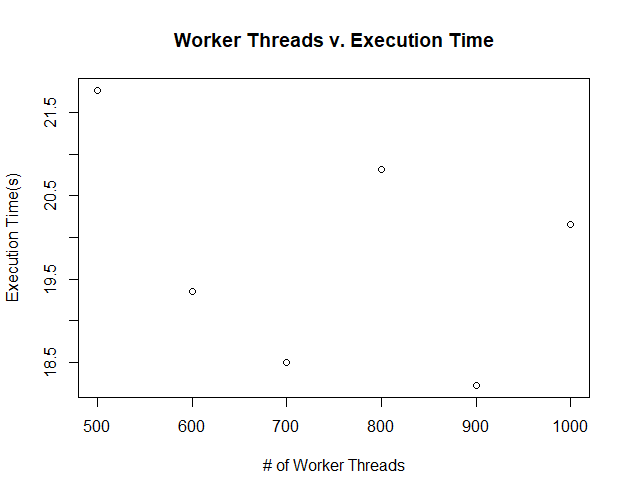
\includegraphics[width=8cm, height=7cm]{PA4_WT_P}
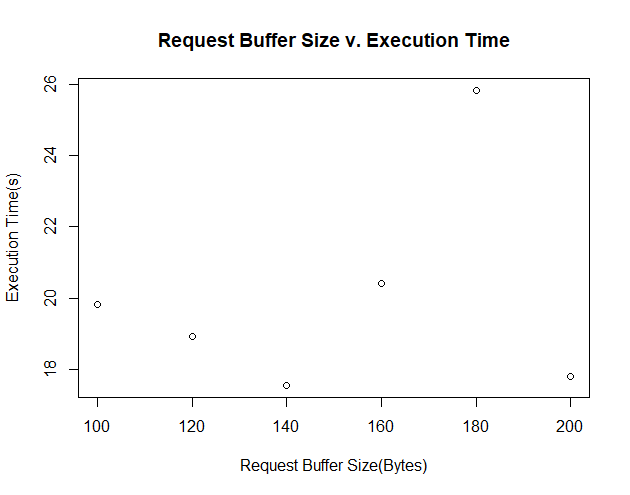
\includegraphics[width=8cm, height=7cm]{PA4_BT-P}
\end{center}

For both worker threads and request buffer size, we see that there is an initial decrease in execution time followed by an increase in execution time for both graphs. The first wave of decreasing execution time for the worker threads is expected since having more threads would mean more threads are running in parallel leading to faster execution time. However, we see an increase in execution time after 700 threads. This can be attributed to the fact that having more threads that the machine can utilize, the execution time will take longer due to more context switches between threads. We see that there is a linear decrease from 500 threads to 700 threads which demonstrates a linear scaling. After that value however, we see undeterministic behavior as there are a lot of factors that affect the execution time such as scheduling, context switches and machine state. We see that this diminishing point after around 600-700 threads as the runtime doesn't improve after increasing the number of worker threads. 

The request buffer size demonstrates a similar trend. The execution time decreases then increases as the request buffer size increases. The request buffer size determines how many requests can be in the buffer at once. If the request buffer is bigger, then more messages can be stored and more threads can run. Therefore, the request buffer size is somewhat correlated to the number of threads. However, once the request buffer size reaches a certain limit then we see that the performance doesn't necessarily get any better since the threads cannot run any faster to consume the messages in the request buffer. Therefore the trend is similar to the worker thread graph. 

\section{Requesting Files}

The plots for file requests with varying values for the number of worker threads and buffer capacity size is shown below. The default number of worker threads is 500 and the default value for the buffer capacity is 256 bytes. We are requesting a file of 100 MB. 

\begin{center}
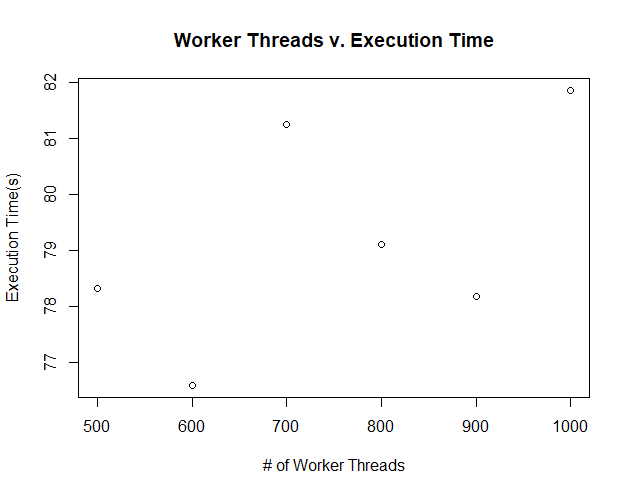
\includegraphics[width=8cm, height=7cm]{PA4_WT_F}
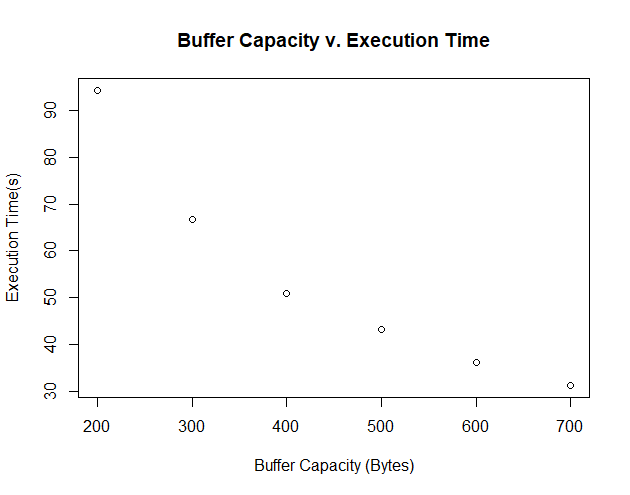
\includegraphics[width=8cm, height=7cm]{PA4_BT_F}
\end{center}

We notice that the number of worker threads doesn't seem to really have that much of an impact on the execution time as there doesn't seem to be any correlation between the number of worker threads and the execution time of the file transfer. This is because the execution time of accessing memory from the disk/SSD is fixed and having more threads doesn't actually speed up this step. Therefore there may be more threads running in parallel but the time it takes to complete the disk IO is still the same regardless of how many threads are running. With a fixed buffer capacity size, we are still doing the same amount of disk IO reads and having more threads doesn't change this number. Therefore, there doesn't really seem to be a linear relationship between the number of worker threads and the execution time of the file transfer. 

When looking at the buffer capacity however, we see a strict decrease in execution time as we increase the buffer capacity. Increasing the buffer capacity decreases the execution time of the file transfer since it causes the program to perform less disk reads which makes the performance better. Having fewer IO reads from the disk, the program runs faster. The relationship from the graph seems to be an inverse relation which makes sense since the execution time is inversely related to the number of disk reads required to transfer the file. 

Demo link: https://youtu.be/vAqmHYfUFNs

\end{document}